\section*{\Large{РЕАЛИЗАЦИЯ}}
\addcontentsline{toc}{section}{РЕАЛИЗАЦИЯ}

При реализации описанной архитектуры была получена следующая структура
проекта(см. рисунок \ref{pic:implementation__packages}).

\begin{figure}[H]
	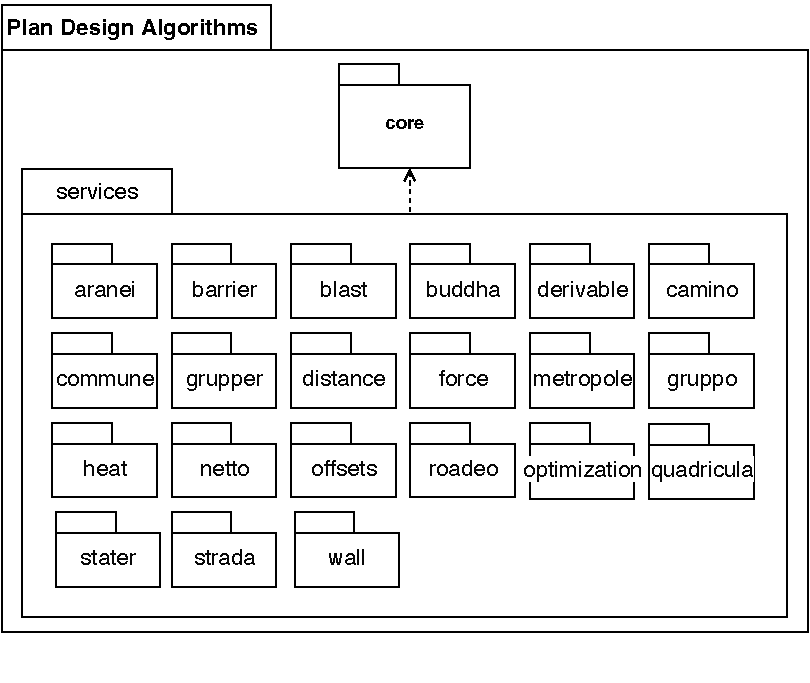
\includegraphics[width=0.6\textwidth]{pictures/packages}
	\caption{Диаграмма пакетов сервиса запуска расчётных задач}
	\label{pic:implementation__packages}
\end{figure}
\vskip 5 mm

Всего получилось 6 python-пакетов, в которых и скрыта основная логика работы.
\begin{enumerate}
    \item \textit{api} -- реализует API сервисы через HTTP. То есть endpoint-ы,
    модели запросов/ответов к серверу, а также взаимодействие с \textit{ITaskRepository} и \textit{ITaskDataManager}
    \item \textit{database} -- обеспечивает взаимодействие с базой данных.
    \item \textit{clients} -- пакеты, в котором находятся клиенты для взаимодействия с сервисами хранилища и сервиса 
    запуска математических методов.
    \item \textit{domain} -- пакет, в котором определены только интерфейсы взаимодействия между модулями программы.
    Непосредственная реализация обозначенных интерфейсов находится в других пакетах.
    \item \textit{execution} -- пакет, в котором находится код, отвечающий за запуск расчётных задач.
    \item \textit{repositories} -- пакет, который обеспечивает логику сохранения/получения сущностей проекта из БД.
\end{enumerate}

\subsection*{\Large{Примеры кода}}
\addcontentsline{toc}{subsection}{Примеры кода}

\begin{lstlisting}[language=Python, caption=main.py, captionpos=b]
from app import startup_app
import uvicorn

if __name__ == '__main__':
    app = startup_app()
    uvicorn.run(app, host="0.0.0.0", port=8080)
\end{lstlisting}

\vskip 10 mm
\begin{lstlisting}[caption=Dockerfile, captionpos=b]]
FROM python:3.8@sha256:4c4e6735f46e7727965d1523015874ab08f71377b3536b8789ee5742fc737059

WORKDIR /app

ENV LC_ALL C.UTF-8
ENV LANG C.UTF-8
ENV N_WORKERS 8

COPY requirements.txt .
RUN pip3 install --no-cache-dir -r requirements.txt

RUN pip3 check

COPY main.py .

COPY /app ./app

ENTRYPOINT /bin/bash -c "gunicorn run_app:app --workers=${N_WORKERS} --bind 0.0.0.0:8080 --worker-class aiohttp.GunicornWebWorker --timeout 0"
\end{lstlisting}

\vskip 10 mm
\begin{lstlisting}[language=Python, caption=domain/model.py, captionpos=b]
class Status(Enum):
    CREATED = "CREATED"
    QUEUED = "QUEUED"
    RUNNING = "RUNNING"
    CANCELLED = "CANCELLED"
    SUCCESS = "SUCCESS"
    FAILURE = "FAILURE"


@dataclass
class Feature:
    id: UUID = UUID(int=0)
    feature_type_id: UUID = UUID(int=0)


@dataclass
class Method:
    id: UUID = UUID(int=0)
    method_type_id: UUID = UUID(int=0)
    status: Status = Status.CREATED


@dataclass
class Calculation:
    id: UUID = UUID(int=0)
    calculation_type_id: UUID = UUID(int=0)
    status: Status = Status.CREATED


@dataclass
class Stage:
    id: UUID = UUID(int=0)
    stage_type_id: UUID = UUID(int=0)
    status: Status = Status.CREATED


@dataclass
class Task:
    id: UUID = UUID(int=0)
    name: str = ""
    task_type_id: UUID = UUID(int=0)
    status: Status = Status.CREATED
\end{lstlisting}
\vskip 10 mm
